\documentclass[conference]{IEEEtran}
\IEEEoverridecommandlockouts
% The preceding line is only needed to identify funding in the first footnote. If that is unneeded, please comment it out.
\usepackage{cite}
\usepackage{amsmath,amssymb,amsfonts}
\usepackage{algorithmic}
\usepackage{graphicx}
\usepackage{textcomp}
\usepackage{xcolor}

\usepackage{threeparttable}
\usepackage{tabularx,booktabs}
\usepackage{siunitx}
  \sisetup{
    table-format=1.3,
    round-mode = places,
    round-precision = 3,
  }
\usepackage{kantlipsum}

\usepackage{capt-of}
\usepackage{cuted}   
\usepackage{booktabs}

\def\BibTeX{{\rm B\kern-.05em{\sc i\kern-.025em b}\kern-.08em
    T\kern-.1667em\lower.7ex\hbox{E}\kern-.125emX}}
\begin{document}

\title{Vergleich verlustfreier Datenkompressionsverfahren auf Bilddaten}

\author{
  \IEEEauthorblockN{Nick Schreiber}
  \IEEEauthorblockA{Technische Hochschule Rosenheim\\
    Master Informatik, Seminar theoretische Informatik\\
    Email: nick.schreiber@stud.th-rosenheim.de}
}

\maketitle

\begin{abstract}

  Die Arbeit vergleicht verlustfreie Datenkompressionsverfahren für Bilddaten.
  Ziel der Arbeit ist es zu untersuchen, ob und warum bestimmte verlustfreie 
  Datenkompressionsverfahren für Bilddaten besser geeignet sind als andere.
  Dazu wird auf die Informationstheorie eingegangen und die theoretischen 
  Grundlagen verschiedener Kompressionsalgorithmen untersucht.
  Ein wichtiger Teil ist der Aufbau und die Besonderheiten von Bildern als 
  Datengrundlage für Kompressionsverfahren.
  Die Arbeit besteht aus einem praktischen Teil, in dem verschiedene Algorithmen 
  zur verlustfreien Datenkompression manuell implementiert und ihre Kompressionsfähigkeit 
  anhand verschiedener Bilder getestet wird.
  Die verglichenen Algorithmen sind Run Length Encoding, Huffman Encoding,
  Lempel-Ziv 1977, Portable Network Graphics und verschiedene Kombinationen der Algorithmen.
  Die Algorithmen werden anhand der Kompressionsrate, der Kompressionszeit und der 
  Dekompressionszeit bewertet.

\end{abstract}


\begin{IEEEkeywords}
  Lossless Image Compression, Information Theory, Compression Algorithms
\end{IEEEkeywords}

\section{Einleitung}

Datenkompression beschreibt ein Verfahren, das zum Ziel hat, eine Nachricht
ohne relevanten Informationsverlust zu verkleinern.
Eine Nachricht ist jede Art von digitalen Daten, z.B. Text, Bild, Audio.
Daten können komprimiert werden, indem Redundanz entfernt oder eine Kodierung angewendet wird.
Daher wird Datenkompression oft als Kodierung bezeichnet.
Kodierung ist ein allgemeiner Begriff, der jede spezielle Darstellung von Daten nach
einem bestimmten Schema umfasst \cite{Ingles}. 

Es gibt zwei Arten der Datenkompression: die verlustbehaftete und die verlustfreie Kompression.
Bei der verlustbehafteten Datenkompression kann eine bestimmte Menge an Information durch die
Kompression verloren gehen, was in Kauf genommen wird, da dadurch die Datenmenge erheblich
reduziert werden kann oder weil die verlorene Informationen für die Anwendung kaum relevant sind.
Das wird auch als Irrelevanzreduktion bezeichnet \cite{Maluck}.
Ein Beispiel für Irrelevanzreduktion kann bei Audiosignalen beobachtet werden.
Der menschliche Hörfrequenzbereich liegt zwischen 20 Hz und 20 kHz \cite{Burke}.
Daher ist es nicht sinnvoll, Frequenzen, die weit außerhalb des hörbaren Bereichs liegen,
in Audiodateien zu speichern.
Bei der verlustfreien Datenkompression wird die Integrität der Daten bewahrt.
Das bedeutet, dass sämtliche Informationen in den komprimierten Daten enthalten sind
und die Originaldaten vollständig rekonstruierbar sind.
In dieser Arbeit wird nur die verlustfreie Datenkompression untersucht, da
Irrelevanzreduktion nicht direkt zum Themengebiet der Datenkompression gehört.

Die Datenkompression von Bildern wird aus verschiedenen Gründen eingesetzt.
Speichernutzung: Unkomprimierte Bilddaten können beträchtlich mehr Speicherplatz beanspruchen.
Übertragungseffizienz: Bei der Übertragung von Bildern über Netzwerke oder das Internet spielt
die Übertragungseffizienz eine entscheidende Rolle.
Wird ein Bild über einen Kanal mit begrenzter Bandbreite übertragen, kann es effizienter sein, 
das Bild zu komprimieren, zu übertragen und beim Empfänger wieder zu dekomprimieren.
Dadurch wird die Übertragungszeit verkürzt und das Bild kann schneller bereitgestellt werden.
Dies führt zu einer höheren Übertragungsrate und einer reduzierten Bandbreitennutzung.


\section{Zielsetzung der Arbeit}

Ziel der Arbeit ist es zu untersuchen, ob und warum bestimmte verlustfreie
Datenkompressionsverfahren für Bilddaten besser geeignet sind als andere.
Dazu werden die theoretischen Aspekte der Kompressionsalgorithmen untersucht.
Außerdem wird untersucht, wie Bilddaten aufgebaut sind und welche Besonderheiten
in den Bilddaten für die Datenkompression genutzt werden können.
Die Arbeit hat einen praktischen Anteil.
Verschiedene Algorithmen zur verlustfreien Datenkompression wurden manuell
implementiert und an unterschiedlichen Bilddaten getestet.
So konnten konkrete Ergebnisse über die Leistungsfähigkeit der Algorithmen gewonnen werden.
Die verglichenen Algorithmen sind Run Length Encoding (RLE), Huffman Encoding,
Lempel-Ziv 1977 (LZ77), Portable Network Graphics (PNG) und verschiedene 
Kombinationen der Algorithmen.
Die Ergebnisse werden interpretiert und mit den theoretischen Erwartungswerten verglichen.

\section{Grundlagen zur Datenkompression}

In der Informatik ist die Datenkompression ein Teilgebiet der Informationstheorie. 
Um zu verstehen, wie verlustfreie Datenkompression funktioniert, muss man einige 
theoretische Grundlagen kennen.

\subsection{Information}

Claude Shannon, der Begründer der Informationstheorie, definiert Information 
als ein Maß für den Informationsgehalt. 
Information ist ein Maß für die Unsicherheit, die durch das Eintreten eines bestimmten 
Ereignisses oder den Erhalt einer Nachricht verringert wird \cite{shannon}.  
Information ist die Mindestanzahl von Bits, die zur Kodierung einer Nachricht verwendet 
werden muss \cite{shannon2}.  
Die Grundidee von Information ist, dass Informationen umso wertvoller sind, je 
unerwarteter oder unwahrscheinlicher sie sind.


\subsection{Entropie}

Die Quantifizierung des Informationsgehalts erfolgt durch die Entropie ($H$).
Formal drückt die Entropie die durchschnittliche Menge an Bits aus,
die benötigt wird, um eine Information zu kodieren \cite{shannon}. 
Die Entropie berücksichtigt die Wahrscheinlichkeiten verschiedener möglicher
Ereignisse und erreicht ein Maximum, wenn alle Ereignisse gleich wahrscheinlich sind,
was auf maximale Unsicherheit hinweist.

\begin{equation}
  \label{eq:entropie}
  H(X) = -\sum_{i=1}^{n} P(x_i) \cdot \log_{2}(P(x_i))
\end{equation}

Formel \ref{eq:entropie} definiert die Entropie mathematisch.
Hierbei steht $H(X)$ für die Entropie der Menge $X$.
$P(x_i)$ steht für die Wahrscheinlichkeit des
Eintretens des Ereignisses $x_i$.
Die Summe wird über alle möglichen Ereignisse
$x_i$ in $X$ gebildet.

Diese Formel beschreibt die durchschnittliche Anzahl von Bits, die 
benötigt werden, um eine Nachricht X zu kodieren.
Wenn die Entropie hoch ist, ist die Unsicherheit groß und es werden mehr 
Bits benötigt, um die Information darzustellen. 
Ist die Entropie niedrig, ist die Unsicherheit gering und es werden weniger 
Bits benötigt. 

Man kann nun einen direkten Zusammenhang zwischen Entropie und Kompression herstellen. 
Niedrige Entropie bedeutet, dass eine Datenmenge strukturiert ist oder Muster aufweist. 
Das bedeutet, dass es wenig Unsicherheit in den Daten gibt und dass die Daten Redundanz 
enthalten. Niedrige Entropie bedeutet, dass die Daten komprimiert werden können.


\subsection{Redundanz und Mutual Information}

Redundanz beschreibt Informationen die in Daten mehrfach vorhanden sind \cite{friedrichs}. 
Vereinfacht kann Redundanz als überflüssige Information betrachtet werden.
Eine hohe Redundanz deutet auf sich wiederholende oder vorhersehbare Muster in den Daten hin.

Um eine Formel für die Redundanz aufzustellen benötigt man die mittlere Codewortlänge.
Die mittlere Codewortlänge gibt den durchschnittlichen Bedarf an Bits pro Symbol in einer
Nachricht an.
Sei $X$ ein Alphabet und $x \in X$.
$C(x)$ bezeichnet das zu $x$ gehörende Codewort.
$l(x)$ bezeichnet die Länge von $C(x)$.
Die mittlere Codewortlänge $L(C)$ einer Nachricht $C(x)$ mit der Wahrscheinlichkeitsverteilung
$p(x)$ ist in Formel \ref{eq:codewortlänge} definiert.

\begin{equation}
  \label{eq:codewortlänge}
  L(C) = \sum_{i}^{|X|} p(x_i) \cdot l(x_i)
\end{equation}

Mit der mittleren Codewortlänge kann die Redundanz des Codes bzw. der Nachricht berechnet 
werden.
Die Formel \ref{eq:redundanz} definiert die Redundanz einer Nachricht.

\begin{equation}
  \label{eq:redundanz}
  R_{\text{Code}} = L(C) - H(X)
\end{equation}

Die Redundanz wird berechnet, indem von der tatsächlichen durchschnittlichen
Anzahl an Bits pro Symbol die theoretisch minimale Anzahl an Bits pro Symbol
abgezogen wird.
Die theoretisch minimale Anzahl an Bits pro Symbol entspricht der enthaltenen
Information und ist gleich der Entropie der Nachricht.
Daraus folgt, dass die Redundanz $\geq$ 0 sein muss.

Mutual Information ist ein quantitatives Maß für die gegenseitige Abhängigkeit zweier
Variablen \cite{shannon}. 
Sie misst, inwieweit die Kenntnis der einen Variablen die Unsicherheit über die 
andere Variable verringert.
Dieses Konzept ist wichtig, um die Struktur der Daten zu verstehen und voneinander 
abhängige Informationen zu erkennen. 

Wenn die Mutual Information zwischen zwei Variablen hoch ist, bedeutet dies, dass die 
Kenntnis der einen Variable wichtige Informationen über die andere Variable liefert.
Hohe Mutual Information bedeutet also, dass zwei Variablen stark voneinander 
abhängig sind.
Das Wissen über den Wert einer Variable trägt bereits wesentlich zur Vorhersage
oder zum Verständnis der anderen Variable bei.

Geringe Mutual Information bedeutet, dass die beiden Variablen weniger überschneidende 
Information teilen.
Das Wissen über den Wert einer Variable trägt nicht zur
Vorhersage oder zum Verständnis der anderen Variable bei.
Dies führt zu einer geringeren statistischen Abhängigkeit der Variablen.

Durch das erkennen von Mutual Information kann gezeigt werden, dass Muster und/ oder
Wiederholungen und dementsprechend Redundanz in den Daten enthalten ist.
Redundanz spielt im Bezug auf Kompression eine wichtige Rolle.
Kompression funktioniert, indem redundante Information identifiziert und eliminiert 
wird, um den Informationsgehalt zu maximieren und die Effizienz der Datenrepräsentation 
zu erhöhen.


\section{Informationstheorie}

Ein wichtiger Punkt in der Informationstheorie ist die Unterscheidung zwischen 
Daten und Information. 
Daten und Information werden umgangssprachlich oft synonym verwendet, was 
nicht korrekt ist. 

Daten sind rohe Fakten oder Symbole, die an sich keine spezifische Bedeutung haben.
Information entsteht durch die Interpretation, Organisation und Strukturierung von Daten, 
wodurch ein sinnvoller Kontext geschaffen wird \cite{pieper}. 
Daten werden zu Informationen, wenn sie für einen bestimmten Zweck verwendet werden können.

Im Zusammenhang mit der Datenkompression ist es wichtig zu verstehen, dass 
nicht alle Daten gleich informativ sind. 
Ein effektiver Kompressionsalgorithmus entfernt redundante und nicht informative 
Teile der Daten. 
Die gesamte Information bleibt jedoch erhalten. 
Die Daten sind dadurch informativer und komprimierter als zuvor.

\subsection{Quellencodierungstheorem/ Source Coding Theorem}

Das Quellencodierungstheorem befasst sich mit der Effizienz der Datenkompression 
und besagt, dass es eine Grenze für die minimale mittlere Codierungslänge gibt, 
die erforderlich ist, um Informationen aus einer bestimmten Quelle 
darzustellen \cite{sharma}. 
Das Quellencodierungstheorem besagt, dass die mittlere Codierungslänge $L$ pro Symbol
für eine gegebene Quelle nicht kleiner sein kann als die Entropie $H$ der Quelle.
Mathematisch in Formel \ref{eq:sct} ausgedrückt.

\begin{equation}
  \label{eq:sct}
  L \ge H
\end{equation}

Die Entropie stellt dabei die untere Schranke für die mittlere Codierungslänge dar.
Daraus wird ersichtlich, dass eine Datenkompression ohne Informationsverlust 
nicht bis ins Unendliche möglich ist. 
Die maximale Kompression ist genau dann erreicht, wenn $L = H$.
Es ist daher nicht sinnvoll, zu versuchen, solche Daten zu komprimieren, da 
dies ohne Informationsverlust nicht möglich ist.

% Vlt. Todo: Schubfachprinzip, Bedeutung von Entropie in diesem Kontext.

\subsection{Kolmogorov Komplexität}

Die Kolmogorov Komplexität ist ein Maß für die Strukturiertheit einer Zeichenfolge.
Sie entspricht der Länge des kürzesten Programms, das die Zeichenfolge 
erzeugen kann \cite{li}. 
Die Kolmogorov Komplexität ist dementsprechend ein Maß für die algorithmische Komplexität
von Information.

Die Kolmogorov Komplexität eines Objekts, z.B. eines Textes, ist die Länge des kürzesten 
Programms, das das Objekt als Ausgabe erzeugt. 
Hier ist ein Beispiel für ein solches Programm. 
Betrachten wir die folgende Zeichenfolge: "AAAAAAAAABBBBBCCCCCC". 
Die Zeichenfolge besteht aus 20 Zeichen (9 x A, 5 x B, 6 x C). 
Mit einem einfachen Programm kann die Zeichenfolge wesentlich kürzer beschrieben 
werden: "9A5B6C". 
Das Programm gibt die Länge der identischen aufeinanderfolgenden Zeichen 
gefolgt von dem Zeichen an. 
Auf diese Weise kann die ursprüngliche Zeichenfolge der Länge 20 in nur 6 
Zeichen dargestellt werden. 
Wir haben ein Programm gefunden, das die Länge der Zeichenfolge erheblich reduziert. 
Die Kolmogorov Komplexität dieser Zeichenfolge ist deutlich kleiner als die 
ursprüngliche Länge der Zeichenfolge. 
Das beweist, dass Strukturen in der Zeichenfolge vorhanden sind.

Es ist wichtig zu beachten, dass die tatsächliche Kolmogorov Komplexität für
allgemeine Zeichenfolge wegen des Halteproblemes nicht praktisch
berechenbar ist \cite{OPPaper}. 
Allerdings können Schätzungen gemacht werden.
Wenn ein Algorithmus gefunden wird, der eine Zeichenfolge in einem kürzeren
Programm darstellt, entspricht die Kolmogorov Komplexität der Zeichenfolge
maximal der Länge des Programms.
Es ermöglicht den Informationsgehalt von Daten in
Bezug auf die kürzest mögliche algorithmische Beschreibung zu verstehen.

% Eine enge Verbindung besteht zur Vorstellung
% der optimalen, universellen Datenkompression – je einfacher die Beschreibung, desto
% effizienter kann die Datenmenge komprimiert werden.
% Dieses Konzept hat weitreichende praktische Anwendungen, von der Identifikation von
% wiederholten Mustern bis hin zur Bewertung von Algorithmeneffizienz.
% Allerdings stehen der Anwendung auch Herausforderungen gegenüber, wie der Unberechenbarkeit
% des absoluten Komplexitätsmaßes und der Schwierigkeit, universelle Algorithmen zu finden,
% die für alle Daten gleichermaßen effizient sind. Das Verständnis der Kolmogorov-Komplexität
% trägt maßgeblich zur Entwicklung fortgeschrittener Datenkompressionsverfahren bei und bietet
% Einblicke in die Grenzen der Komprimierbarkeit von Informationen.

% Anforderungen an Daten, damit diese komprimierbar sind
\subsection{Datenanforderungen, Komprimierbarkeit}

Daten lassen sich in verschiedene Gruppen einteilen. 
Auf der einen Seite stehen die strukturierten Daten und auf der anderen 
Seite die unstrukturierten Daten. 
Strukturierte Daten sind Daten, die wiederkehrende oder vorhersehbare Muster enthalten. 
Die Entropie der Daten ist gering. Tabellen sind ein Beispiel für strukturierte Daten. 
Unstrukturierte Daten sind Daten, die keine wiederkehrenden oder vorhersehbaren 
Muster enthalten. Die Datenentropie ist hoch. 
Ein Beispiel für unstrukturierte Daten sind zufällig generierte Daten. 

Strukturierte Daten enthalten in der Regel mehr Redundanz als unstrukturierte Daten. 
Dies liegt daran, dass die maximal mögliche Kompression der Information in den Daten 
gleich der Entropie ist. 
Daten können theoretisch maximal auf das Niveau der Entropie der Daten komprimiert werden.
Strukturierte Daten mit niedriger Entropie haben eine tiefere Grenze als 
unstrukturierte Daten.
Daher können strukturierte Daten in der Regel stärker komprimiert werden als 
unstrukturierte Daten.

\subsubsection{Vorverarbeitung}

Eine Möglichkeit, unstrukturierte Daten in strukturiertere Daten umzuwandeln, ist 
die Vorverarbeitung der Daten. 
Eine solche Vorverarbeitung ist in der Regel eine Normalisierung oder Filterung 
der Daten. 
Wichtig ist, dass der Vorverarbeitungsschritt umkehrbar ist. 
Eine Möglichkeit, Daten für die Kompression vorzubereiten, wird in dieser Arbeit 
anhand des PNG-Algorithmus gezeigt. 
PNG verwendet Datenfilterung.

\subsubsection{Limitationen}

Ein Beispiel für maximal unstrukturierte Daten, die scheinbar nicht komprimierbar 
sind, sind normalverteilte Zufallszahlen. 
"The Random Compression Challenge" von Mark Nelson \cite{nelson} untersucht 
genau dieses Problem. 
Ziel der Challenge ist es, eine Datei zu komprimieren, die etwa ein halbes Megabyte groß ist.
Die Datei besteht aus einer Millionen gleichverteilter Zufallszahlen, die aus dem 
Buch "A Million Random Digits with 100,000 Normal Deviates" \cite{amilli} stammen.

Es gibt zwei Wege, die Challenge zu gewinnen.
Die erste Möglichkeit besteht darin, die Kolmogorov Komplexität zu verwenden und 
ein Programm zu schreiben, das die Originaldatei erzeugt.
Die größe des Programms muss kleiner sein, als die zu komprimierende Datei.
Das Programm muss kleiner sein als die zu komprimierende Datei. Es muss gezeigt werden, 
dass die Kolmogorov Komplexität kleiner ist als die Größe der Datei selbst.

Die andere Möglichkeit besteht darin, ein System zu entwickeln, das in der Lage 
ist, Dateien mit normalverteilten Zufallszahlen zu komprimieren und die komprimierte 
Datei vollständig zu dekomprimieren. 
Die Größe des Systems spielt dabei keine Rolle, da das System mehr als eine Datei 
erfolgreich komprimieren und dekomprimieren muss. 
Es ist bewiesen, dass dieser Ansatz unmöglich ist \cite{nelson}. 
Der Grund dafür ist, dass die Entropie der Größe der Datei selbst entspricht und 
nicht ohne Informationsverlust reduziert werden kann.

Bisher hat noch niemand die Challenge gewonnen. 
Das ist nicht verwunderlich, denn die zweite Möglichkeit zu gewinnen ist 
nachweislich unmöglich. 
Dagegen ist die erste Möglichkeit mit der Kolmogorov Komplexität nur wahrscheinlich 
unmöglich. 
Das bedeutet, dass es zwar eine Lösung geben könnte, diese aber nach derzeitigem 
Stand unwahrscheinlich ist. 
Die Herausforderung ist ein perfektes Beispiel dafür, warum es sinnvoll ist, die 
Daten zu kennen, die man komprimieren möchte. 
Sie zeigt die Grenzen der Datenkompression auf.


\section{Aufbau und Struktur von Bilddaten}

Dieser Abschnitt befasst sich mit dem Aufbau und der Struktur von Bilddaten. 
Es gibt verschiedene Möglichkeiten, Bilddaten zu speichern und darzustellen. 
In dieser Arbeit werden die Bilder in Form einer Rastergrafik/ Bitmap, dem RGB Format, 
gespeichert. 
Eine Rastergrafik ist eine pixelbasierte Darstellung eines Bildes. 
Die Auflösung eines Bildes gibt an, wie viele Pixel in der Breite und Höhe vorhanden sind. 
Ein Pixel ist die kleinste diskrete Einheit eines digitalen Bildes. 

Das RGB Format ist eine Möglichkeit, Farbinformationen in digitalen Bildern darzustellen 
und zu speichern. 
RGB steht für die Farben Rot (R), Grün (G) und Blau (B). 
Es ist ein additives Farbmodell und jede Farbe wird durch eine Kombination der drei 
Grundfarben, einschließlich Weiß und Schwarz, erzeugt \cite{rite}.

Ein Beispielbild mit einer Auflösung von 800 Pixel Breite und 800 Pixel Höhe wird 
im RGB Format in einer Matrix gespeichert. 
Die entsprechende Matrix hat die Größe (800, 800, 3), (Breite, Höhe, Farbkanäle). 
Die dritte Dimension ist die Zahl der Farbkanäle. 
Für jeden Pixel werden drei Werte gespeichert, die die Farbe des Pixels beschreiben. 
Der erste Wert ist der Rotanteil, der zweite der Grünanteil und der dritte der Blauanteil. 
Das RGB Format verwendet normalerweise 8 Bit pro Farbkanal, was eine Farbtiefe von 24 Bit 
pro Pixel ergibt. 
Jeder Farbwert eines Pixels hat 8 Bit bzw. 1 Byte Speicherplatz zur Verfügung und 
kann Werte zwischen 0 und 255 annehmen.

Bilder im RGB Format sind nach einem bestimmten Schema aufgebaut, weshalb
Strukturen in den Bilddaten entstehen.
Diese Strukturen können bei der Datenkompression helfen, die Bilder zu komprimieren.
Eine Struktur im RGB Format ist die Darstellung von Nichtfarben
wie Schwarz und Weiß.
Um Schwarz oder Weiß darzustellen, muss ein Pixel für alle drei Farbkanalwerte entweder 
den Wert 0 oder 255 annehmen. 
Um reine Farben wie Rot darzustellen, wird nur ein Pixelwert für den Rotanteil 
benötigt, während die Grün- und Blauanteile auf Null gesetzt werden. 
Ebenso gibt es viele Farbmischungen, bei denen eine der Grundfarben nicht benötigt 
wird und deren Anteil im Pixel daher auf 0 gesetzt wird. 
Diese Strukturen entstehen, wenn das Bild im RGB Format vorliegt. 
Eine weitere Struktur, die in den meisten Bildern vorkommt, ist, dass benachbarte 
Pixel meist ähnliche oder die gleiche Farbe haben. 
Dies hängt damit zusammen, dass es in Bildern häufig Regionen gibt, die zu einem 
Objekt oder Bildteil gehören und eine homogene Farbe besitzen.

Diese Strukturen und Wiederholungen in den Bilddaten können ausgenutzt werden um die
Daten zu komprimieren.
Bei der Datenkompression ist es entscheidend, welche Algorithmen diese Redundanzen, 
die strukturell in den Bildern enthalten sind, erkennen und ausnutzen können.

% Todo vlt Vergleich mit Textdaten, Unterschiede!!!!, hier oder später aber wäre interessant

\section{Messbarkeit der Kompressionsalgorithmen}

Es ist wichtig, Kriterien festzulegen, anhand derer die Algorithmen bewertet werden können.
Eine Messbarkeit ist notwendig, um Datenkompressionsalgorithmen und deren Ergebnisse
vergleichen zu können und um zu entscheiden, was ein guter Kompressionsalgorithmus ist.

Ein Kompressionsalgorithmus arbeitet in mehreren Schritten. 
Schritt 1 ist die Vorverarbeitung der zu komprimierenden Daten. 
Dieser Schritt ist optional und transformiert die Originaldaten. 
Schritt 2 ist die Komprimierung der Daten. 
In diesem Schritt wird der für die Kompression spezifische Algorithmus angewendet,
um die Daten zu komprimieren.
Das Ergebnis sind komprimierte Daten und optional je nach Algorithmus spezifische 
Zusatzinformationen. 
Schritt 3 ist die Dekompression der komprimierten Daten. 
Dabei wird die Kompression rückgängig gemacht. 
Schritt 4 ist die Dekompression des Vorverarbeitungsschrittes, falls verwendet. 
Die Daten, die diesen Zyklus durchlaufen, sind mit den Originaldaten identisch, da 
es sich um verlustfreie Kompressionsalgorithmen handelt. 
Um die Qualität eines Kompressionsalgorithmus konkret bewerten zu können, werden 
die folgenden drei Kriterien festgelegt, anhand derer die Bewertung vorgenommen wird.


\subsection{Kompressionsrate}

Eine Möglichkeit, die Effizienz eines Datenkompressionsverfahrens zu beurteilen, 
besteht darin, die Datengröße der komprimierten Daten (nach Schritt 2, einschließlich 
Zusatzinformationen, falls vorhanden) zu betrachten. 
Die Datengröße kann in der Maßeinheit Bit oder Byte bestimmt werden und gibt an, wie 
viel Speicherplatz die Daten benötigen. 
Ein Maß dafür, wie stark die Daten im Vergleich zu den Originaldaten mit dem 
jeweiligen Algorithmus komprimiert werden können, ist die Kompressionsrate. 
Die Kompressionsrate ergibt sich aus dem Verhältnis der Größe der ursprünglichen, 
unkomprimierten Daten zur Größe der komprimierten Daten.
Sie wird in Prozent angegeben und ist in der Formel \ref{eq:komprate} angegeben.

\begin{equation}
  \label{eq:komprate}
  \text{Kompressionsrate} = \left(1 - \frac{\text{Größe komp. Daten}}{\text{Größe unkomp. Daten}}\right) \times 100 \%
\end{equation}

Je höher die Kompressionsrate, desto stärker hat der Algorithmus die Daten komprimiert. 
Eine Kompressionsrate von 100 \% kann nur erreicht werden, wenn die Originaldaten keine 
Informationen enthalten und daher leer sind. 
Ein Wert von 0 \% bedeutet, dass keine Kompression stattgefunden hat und die komprimierten 
Daten genauso groß sind wie die Originaldaten. 
Ein negativer Wert ist möglich und zeigt an, dass die komprimierten Daten mehr 
Speicherplatz benötigen als die Originaldaten. Dies bedeutet, dass der Algorithmus 
die Originaldaten nicht erfolgreich komprimieren konnte. 
Die Kompressionsrate kann Werte im Bereich $(-\infty, 100]$ annehmen. 
Die Bewertung mit der Kompressionsrate ist datenabhängig und wird konkret
ermittelt.
Das Bedeutet die zu komprimierenden Daten sind entscheidend.


\subsection{Kompressionszeit}

Ein weiteres Kriterium zur Bewertung von Datenkompressionsalgorithmen ist die Kompressionszeit. 
Die Kompressionszeit gibt an, wie lange ein Algorithmus benötigt, um aus den Originaldaten 
komprimierte Daten zu erzeugen. 
Sie misst die kombinierte Zeit für die Vorverarbeitung (Schritt 1) und die Anwendung 
des Kompressionsalgorithmus (Schritt 2). 
Die Kompressionszeit wird in Sekunden gemessen. 
Eine Messung erfolgt immer genau an einem Input, der komprimiert wird. 
Es werden also konkrete Werte gemessen. 
Durch das Messen und Vergleichen von unterschiedlich großen Eingangsdaten können konkrete 
Aussagen über die Kompressionszeit in Abhängigkeit von der Größe der Eingangsdaten 
gemacht werden. 

Die konkreten Ergebnisse der Kompressionszeit können mit der theoretisch erwarteten 
Laufzeit der Algorithmen verglichen werden. 
Die theoretische Laufzeit eines Algorithmus wird in der O-Notation angegeben. 
Die O-Notation beschreibt die obere Grenze des Wachstumsverhaltens der Laufzeit eines 
Algorithmus in Bezug auf eine wachsende Eingabe \cite{chivers}.  
Aus den praktischen Messungen und der theoretischen Vorhersage können Rückschlüsse auf 
die implementierten Algorithmen gezogen werden.
% vlt noch mehr O-Notation

\subsection{Dekompressionszeit}

Die Dekompressionszeit ist ein weiteres Maß zur Bewertung von 
Datenkompressionsalgorithmen. 
Sie gibt an, wie viel Zeit ein Algorithmus benötigt, um aus komprimierten Daten 
wieder die ursprünglichen Daten zu erzeugen. 
Sie misst die kombinierte Zeit für die Dekompression (Schritt 3) und die Umkehrung 
der Vorverarbeitung (Schritt 4). Die Dekompressionszeit wird in Sekunden gemessen. 
Die Messungen erfolgen wie bei der Kompressionszeit an konkreten Daten.


\subsection{Abwägung der Messkriterien}

Nach der Definition der drei Messkriterien, anhand derer die Kompressionsalgorithmen 
verglichen werden, können diese zusätzlich gewichtet werden. 
Je nach Anwendungsfall sind die Messkriterien von unterschiedlicher Bedeutung. 
In den folgenden Abschnitten werden drei Beispiele für unterschiedliche Anwendungen 
und Gewichtungen der Kriterien vorgestellt.

Beispiel 1, Echtzeitanwendungen:
Bei der Übertragung von Daten über ein Netzwerk mit begrenzter Bandbreite ist es für 
Echtzeitanwendungen sinnvoll, die Daten vor der Übertragung zu komprimieren.
Dadurch wird nur eine geringere Bandbreite benötigt und die Übertragung der
Daten erfolgt schneller.
Auf der Empfängerseite müssen die Daten möglichst schnell dekomprimiert werden.
Für diesen Anwendungsfall ist die Kompressions- und Dekompressionszeit entscheidend.
Die Kompressionsrate spielt eine untergeordnete Rolle.

Beispiel 2: Ressourcen im Internet: 
Für eine Webseite, die Ressourcen wie z.B. Bilder anzeigen soll, ist es 
wichtig, dem Besucher der Webseite die Ressourcen so schnell wie möglich zur 
Verfügung zu stellen. 
Da das Internet ein Netzwerk mit begrenzter Bandbreite ist, ist es sinnvoll, die 
Ressourcen komprimiert zu senden und beim Besucher zu dekomprimieren. 
Für diesen Anwendungsfall spielt die Kompressionszeit keine Rolle, da die Ressourcen 
bereits in vorkomprimierter Form vorliegen können. 
Entscheidend ist hier die Dekompressionszeit und sekundär die Kompressionsrate.

Beispiel 3, Archivierung:
Archivierung ist das langfristige Speichern von Daten.
Auf die Daten wird nur selten zugegriffen.
Entscheidend ist, dass die Daten möglichst wenig Speicherplatz benötigen,
um möglichst viele Daten speichern zu können.
Für diesen Anwendungsfall ist das Messkriterium Kompressionsrate wichtig.
Die Zeit für die Kompression und Dekompression der Daten spielt aufgrund der 
seltenen und nicht zeitkritischen Datenzugriffe keine Rolle.

Die Beispiele zeigen, dass es sinnvoll ist, die Datenkompressionsalgorithmen 
anhand der drei Kriterien zu vergleichen, da diese je nach Anforderung unterschiedlich 
wichtig sind.


\section{Aufbau des praktischen Versuchs}

Ziel des praktischen Versuchs ist es, verschiedene Datenkompressionsalgorithmen 
anhand von Bildern zu vergleichen. 
Nicht alle Algorithmen, die verglichen werden, sind für die Kompression von Bildern geeignet. 
Die Bilder müssen vorbereitet und in das richtige Format gebracht werden.

\begin{figure}[h]
  \centering
  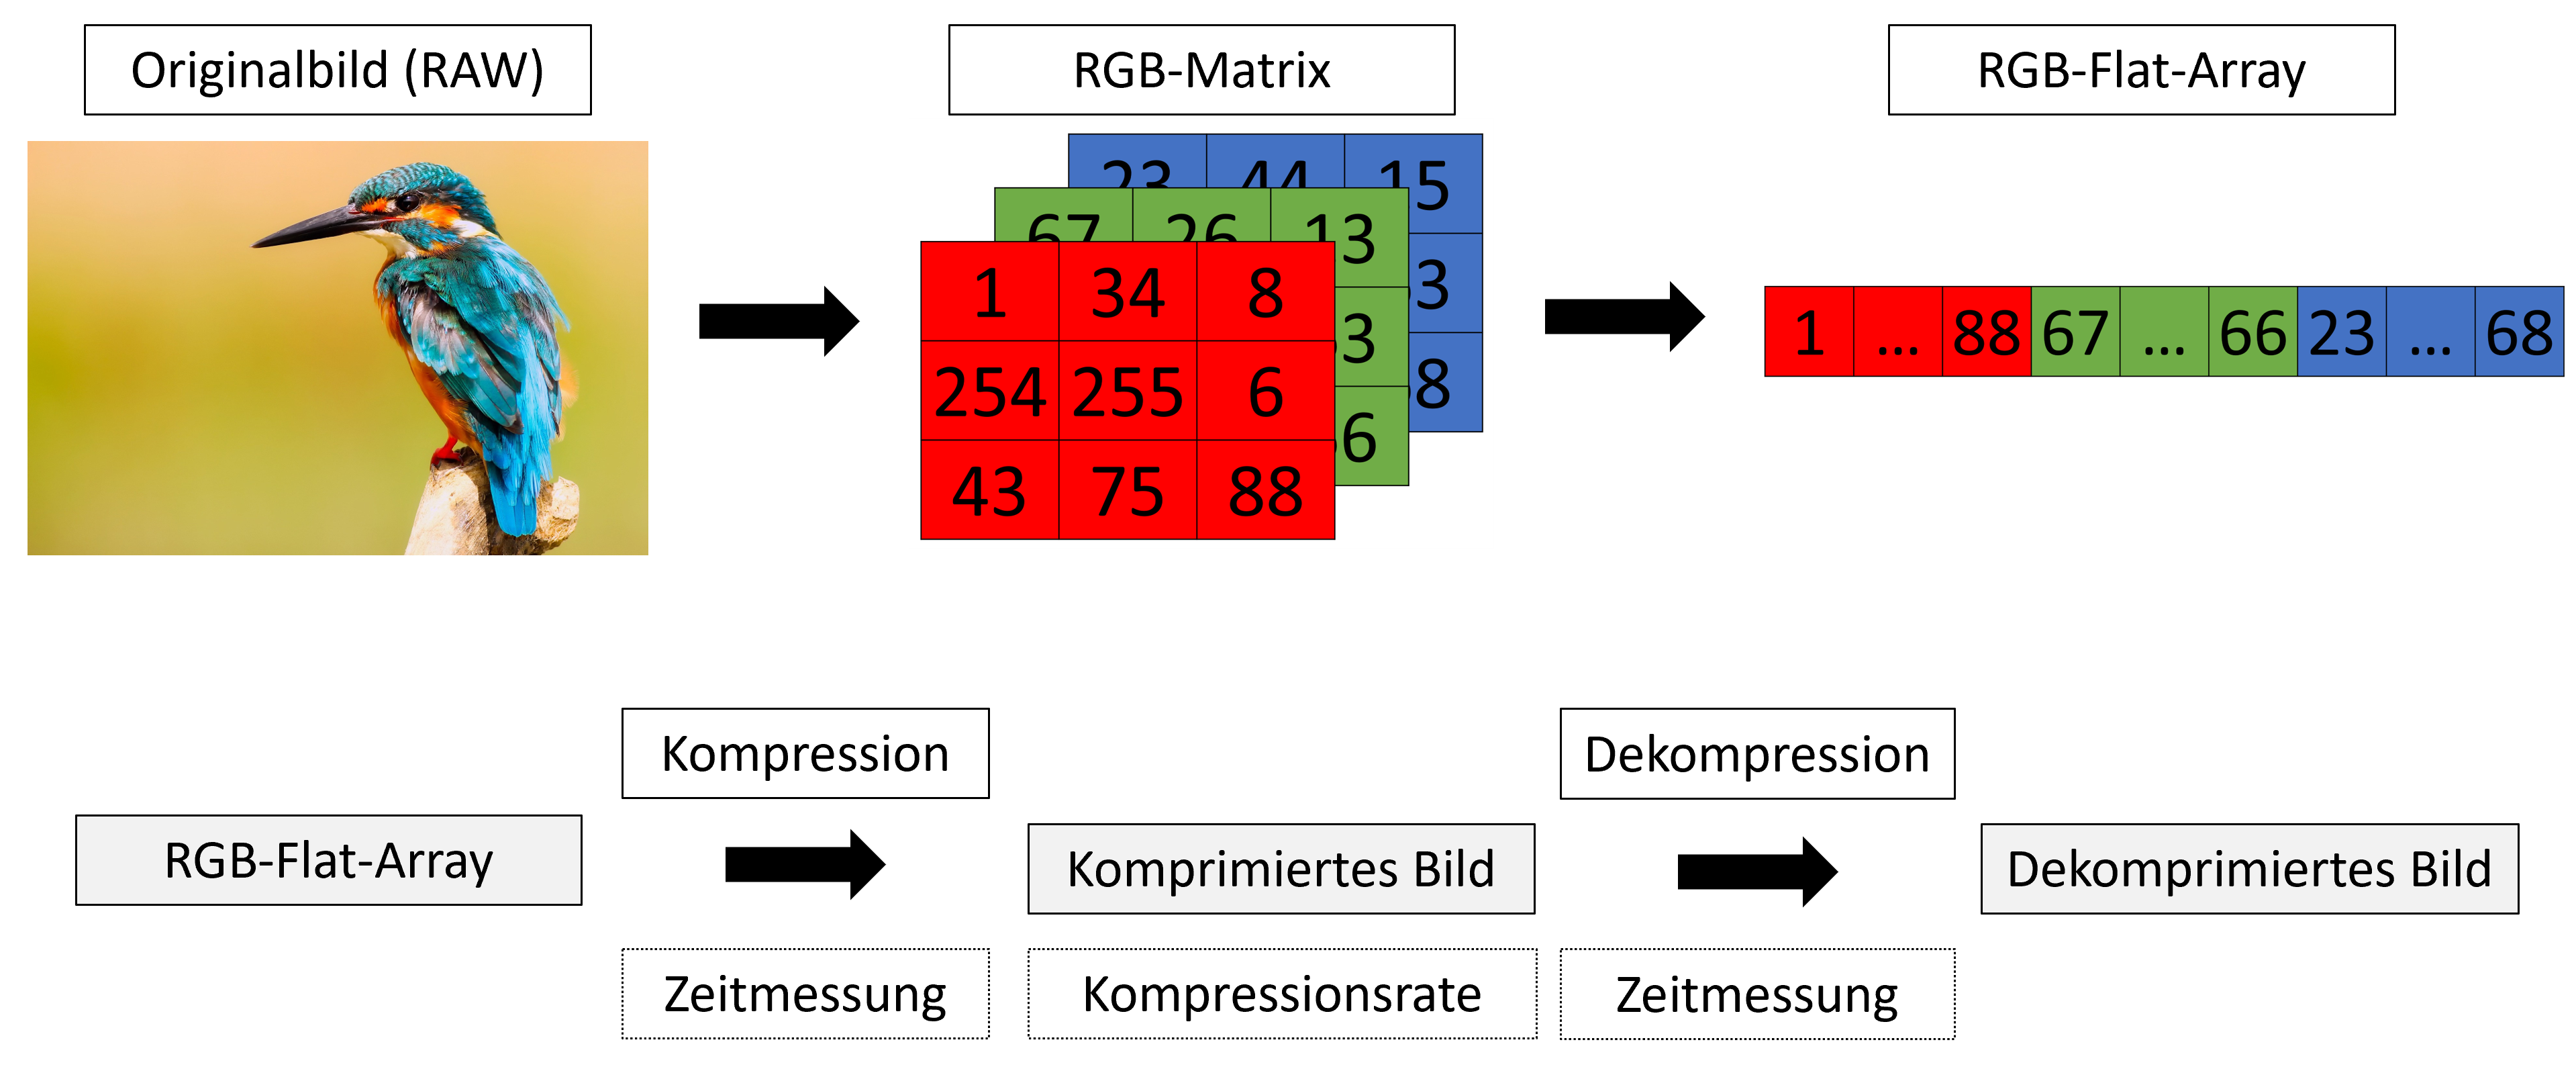
\includegraphics[width=\columnwidth]{./images/Idea.png}
  \caption{Umsetzung des Versuchs}
  \label{fig:idea}
\end{figure}

Abbildung \ref{fig:idea} zeigt den Aufbau des Versuchs.
Die erste Zeile zeigt, wie das Eingangsbild in das benötigte Format umgewandelt
wird.
Das Originalbild, das komprimiert werden soll, ist unkomprimiert und unbearbeitet. 
Es wird im ersten Schritt in eine RGB Matrix umgewandelt.
Die Konvertierung vom Originalbild zur Matrix, aber auch von der Matrix zum Originalbild 
ist möglich und eindeutig umkehrbar.
Die Matrix hat die Form (Pixelbreite Originalbild, Pixelhöhe Originalbild,
3 Farbkanäle).
Jeder der drei Farbkanäle (rot, grün, blau) beschreibt eine zweidimensionale Matrix,
die für jeden Pixel den Wert der entsprechenden Farbe angibt.
Im nächsten Schritt wird die Matrix in eine flache Liste umgewandelt.
Dazu werden alle Werte der Farbkanäle aneinandergereiht.
Zuerst alle Werte des Farbkanals für Rot, dann für Grün, dann für Blau.

Einige der verglichenen Kompressionsalgorithmen sind für Textdaten konzipiert.
Textdaten sind eindimensionale Daten, während Bilddaten je nach Darstellung
zweidimensional sind.
Mit den oben beschriebenen Schritten wird ein Bild in eine eindimensionale
Form umgewandelt.
Die Algorithmen können mit dieser Darstellung eines Bildes arbeiten.

Die untere Zeile der Abbildung \ref{fig:idea} beschreibt den Programmablauf. 
Die Eingabe für den Kompressionsalgorithmus ist die eindimensionale RGB Liste. 
Der Algorithmus komprimiert die Eingabedaten und erzeugt die komprimierte 
Darstellung des Bildes, hier Komprimiertes Bild genannt. 
Die Zeit vom Start des Algorithmus bis zum komprimierten Bild wird gemessen 
und als Kompressionszeit gespeichert. 
Aus den komprimierten Daten wird die Kompressionsrate nach der 
Formel \ref{eq:komprate} berechnet. 
Im nächsten Schritt dekomprimiert der Algorithmus die komprimierten Daten 
und erzeugt die ursprüngliche RGB Liste. 
Die Zeit für die Dekompression wird als Dekompressionszeit gespeichert.

% Umsetzung in Python, high level programming language, schnell umsetzbar, aber nicht
% Laufzeitoptimiert
% Vereinfachungen/ Annahmen getroffen:
% - keine Optimierungen der Algorithmen,
% - 8-Bit Farbinformationen,


% Todo ab hier!!!!!!!!!!!!!!!!!!!!!!!!!!!!!!!!!!!!!!!!!!

\section{Vorstellung der Kompressionsalgorithmen}

In diesem Abschnitt werden die verglichenen Datenkompressionsalgorithmen
mit ihren jeweiligen Spezifikationen vorgestellt.
Für den praktischen Teil der Arbeit wurden alle
Algorithmen in der Programmiersprache Python manuell implementiert
(GitHub Repo \cite{nick}).
Python ist eine Hochsprachen-Programmiersprache, die es ermöglicht,
die verschiedenen Algorithmen entsprechend ihrer Spezifikationen zu implementieren.
Die Sprache Python wurde gewählt, da sie eine schnelle Implementierung ermöglicht.
Python ist eine interpretierte Sprache und nicht auf die Laufzeit von Programmen
optimiert. \cite{nadav}
In den Implementierungen der Algorithmen wurden keine Laufzeitoptimierungen der
Algorithmen vorgenommen.
Es geht in dem Versuch darum die Kompressionsalgorithmen untereinander zu
vergleichen und nicht eine jeweils beste Lösung zu implementieren.


\subsection{Run Length Encoding - RLE}

RLE, auf deutsch Lauflängenkodierung, ist eine der einfachsten Kompressionsalgorithmen.
Die Grundidee besteht darin, aufeinanderfolgende gleiche Elemente durch
eine einzige Instanz des Elements und die Anzahl der Wiederholungen zu ersetzen.
RLE ist besonders effektiv, wenn in den Daten viele aufeinanderfolgende
gleiche Zeichen vorhanden sind.
RLE ist eine Encoding Algorithmus und versucht die Kompression der Daten
durch eine andere Struktur der Daten zu erreichen.
RLE ist besonders effektiv, wenn in den Daten viele aufeinanderfolgende
gleiche Zeichen vorhanden sind, da diese Redundanz durch das Zeichen und die
Anzahl an wiederholungen repräsentiert werden kann.

Die Daten die komprimiert werden sollen sind Ganzzahlwerten zwischen 0 und 255.
Ein Ganzzahlwert ist ein Element und benötigt ein Byte Speicher.
Die Anzahl der gleichen hintereinanderfolgenden Elemente ist die Lauflänge.
Die RLE Darstellung der Daten ist: (Element, Lauflänge)*.
Über dieses Encoding versucht RLE Daten zu komprimieren.

Es gibt viele leicht abweichende Spezifikationen um eine Lauflänge
von einem Elementen abgrenzbar zu machen.
Es gibt die Möglichkeit bestimmte Trennsymbole zu verwenden.
Die Spezifikation die für den Versuch gewählt wurde, ist,
dass die Lauflänge immer eine bestimmte Anzahl an Bits verwendet.
Die Anzahl an Bits entspricht genau der minimalen Anzahl an Bits,
mit der die maximale Lauflänge repräsentiert werden kann.
Diese Bitanzahl wird benötigt um die Encodierten Daten zu Decodieren.
Sie wird als ein Byte Metadaten mitgespeichert.
Weitere Metadaten sind die
Auflösung des Bildes um aus den eindimensionalen Daten das Originalbild
zu rekonstruieren.

Nach der gewählten Implementierung hat
RLE für das Encoding, bzw. den Kompressionsschritt, eine
Laufzeitkomplexität von $O(n)$, n entspricht der Länge der Ausgangsdaten.
Für das Decoding, bzw. den Dekompressionsschritt hat RLE eine
Laufzeitkomplexität von $O(m)$, m ientspricht der Länge der encodierten Daten. \cite{nick}
% todo repo vorbereiten

\subsection{Huffman Codierung}

Die Huffman Codierung beruht auf der Idee, häufig vorkommende Zeichen in einem Datenstrom
mit kürzeren Binärcodes zu repräsentieren, während seltener vorkommende Zeichen längere Codes
erhalten.
Der Algorithmus beginnt mit einer Analyse der Häufigkeit jedes Zeichens in den Daten.
Anschließend wird ein Huffman Baum erstellt, wobei jedem Zeichen ein Blatt zugeordnet wird.
Die Erstellung des Baums erfolgt so, dass häufige Zeichen kürzere Pfade im Baum haben.
Jedes Zeichen erhält einen eindeutigen Binärcode.
Die Zuordnung der Binärcodes erfolgt durch das durchschreiten des Huffman Baums.
Eine Linksabzweigung im Baum entspricht einem Binärwert "0", rechts entspricht "1".
Für die Decodierung der Encodierten Daten wird der Huffman Baum benötigt.
Dieser muss als Metadaten mitgespeichert werden.

Die Datenkompression erfolgt durch Redundanzminimierung mittels Analyse
der Zeichenhäufigkeiten und entsprechender Kodierung.
Die Huffman Codierung ist besonders effektiv auf Daten, in denen die
Wahrscheinlichkeiten der auftretenden Zeichen stark variieren.
\cite{moffat}

Nach der gewählten Implementierung hat
die Huffman Codierung für das Encoding, bzw. den Kompressionsschritt, eine
Laufzeitkomplexität von $O(n log n)$, n entspricht Länge der Ausgangsdaten.
Für das Decoding, bzw. den Dekompressionsschritt hat die Huffman Codierung eine
Laufzeitkomplexität von $O(m)$, m entspricht der Länge der encodierten Daten. \cite{moffat}

\subsection{Lempel-Ziv 1977 - LZ77}

Die Idee des LZ77 Algorithmus besteht darin, wiederkehrende Muster
in einem Datenstrom zu erkennen und durch Verweise auf bereits übertragene Daten zu ersetzen.
Der Algorithmus funktioniert, indem er eine sogenannte "Sliding Window" über den
Datenstrom bewegt.
nnerhalb dieses Fensters wird nach wiederkehrenden Sequenzen gesucht.
Wenn eine solche Sequenz gefunden wird, wird sie durch einen Verweis auf die
vorherige Instanz der Sequenz ersetzt, wobei die Position und Länge der vorherigen Instanz
angegeben werden.

Die Datenkompression erfolgt durch das entfernen von Redundanz durch das verweisen auf bereits
bekannte Zeichensequenzen.
Der Algorithmus ist besonders effektiv für Daten mit wiederkehrenden Mustern.

Nach der gewählten Implementierung hat
LZ77 für den Kompressionsschritt eine Laufzeitkomplexität von
$O(n * s)$, n entspricht der Länge der Ausgangsdaten und s entspricht der
Größe des Sliding Window.
Für den Dekompressionsschritt hat LZ77 eine
Laufzeitkomplexität von $O(m * s)$, m entspricht der Länge der encodierten Daten, s entspricht der
Größe des Sliding Window. \cite{nick}

Eine Spezifikation die für LZ77 bei der Implementierung getroffen wurde ist,
dass die Größe des "Sliding Window" auf 100 Zeichen gesetzt wurde.
Eine größere Größe des Sliding Window ist mit Python ohne
weitere optimierungen nicht für große Datenmengen geeignet, da die Laufzeit
sonst übermäßig ansteigt.

\subsection{Deflate Algorithmus}
\label{deflate}

Der Deflate Algorithmus kombiniert LZ77 und Huffman Codierung.
Die Daten werden im ersten Schritt mit LZ77 codiert.
Die Codierten Daten werden im nächsten Schritt mit Huffman weiter codiert.
Zum Decodierung der komprimierten Daten werden die Decodierungsschritte von Huffman
und LZ77 benötigt.
Die Laufzeitkomplexität der Kompression und Dekompression entsprechen der von
LZ77, da $O(n + n * s) = O(n * s)$.

\subsection{Portable Network Graphics Algorithmus - PNG}

PNG ist ein Format um Bilder zu speichern.
Der PNG Algorithmus ist ein verlustfreies Bildkompressionsformat.
PNG und alle Spezifikationen sind im Standard von W3C definiert. \cite{w3c}

Der PNG Algorithmus kann in drei großen Schritten zusammengefasst werden.
Schritt 1 ist ein Vorverarbeitungsschritt der Bilddaten die mit Hilfe von
Filtern für den Kompressionsschritt vorbereitet werden.
Schritt 2 ist der Kompressionsschritt.
Die Daten werden mit Hilfe des Deflate Algorithmus komprimiert.
Schritt 3 ist ein Cyclic Redundancy Check zur Integritätsüberprüfung.


\subsubsection{Vorverarbeitung der Bilder: Filtern}

Der Vorverarbeitungsschritt, bzw. das Filtern, dient dazu, lokale Korrelationen und
Muster in den Bilddaten zu erzeugen.
Die Idee dabei ist es, dass der nachfolgende Kompressionsschritt
auf den gefilterten Daten besser funktioniert als auf den ungefilterten.
Der Vorverarbeitungsschritt versucht Redundanz in den Daten zu erzeugen, welche
von dem Deflate Algorithmus entfernt werden kann.

Beim Filtern wird jeder Farbkanal eines Bildes einzeln betrachtet.
Das Filtern erfolgt zeilenweise.
Ein Filter wird auf jedem Pixel einer Zeile angewendet.

Für jede Zeile kann genau ein Filtertyp gewählt werden.
Es gibt fünf verschiedene Filtertypen, die auf jeder Zeile
des Bildes angewendet werden können: None, Sub, Up, Average und Paeth.
Jeder dieser Filtertypen transformiert die Werte in einer Reihe Pixelweise nach einer spezifischen
Funktion.
Die verwendeten Funktionen beschreiben die Pixelwerte meist in Relation zu benachbarten Pixel.

\begin{enumerate}
  \item Der None Filter verändert den Inhalt einer Zeile nicht.
  \item Der Sub Filter berechnet die Differenzen der in einer Zeile aufeinanderfolgenden Pixel.
  \item Der Up Filter berechnet die Differenze des Pixelwertes in der aktuellen Zeile mit
        dem Pixelwert der Zeile darüber.
  \item Der Average Filter berechnet die durchschnittliche Differenz eines Pixelwertes zum
        Pixelwert links und darüber.
  \item Der Paeth Filter berechnet die Differenzen zum Pixelwert links, darüber, darüber links und nimmt den
        minimalen Wert der Differenzen der drei Pixelnachbarn.
\end{enumerate}

Die ausführlichen Spezifikationen der Filter finden sich in den W3C Spezifikationen \cite{w3c} unter
Abschnitt 9.

Da für jede Zeile nur ein Filtertyp angewendet werden kann, muss für die jeweilige
Reihe der best passende Filtertyp gewählt werden, um die erzeugte Redundanz zu maximieren.
Die Auswahl erfolgt auf Basis einer Heuristik.
Die Heuristik zielt darauf ab den Filtertyp zu wählen, der am meisten Redundanz erzeugt.
Die Heuristik wählt den Filtertyp für den die Summe aller Werte in einer Reihe
am geringsten ist.
Es gibt keine Garantie, dass der gewählte Filtertyp zu der besten Datenkompression
führt.
Um die tatsächlich beste Kombination an Filtertyp pro Zeile zu finden müssten alle
Kombinationen ausprobiert werden.
Das ist allerdings nicht möglich, da die Anzahl an Kombinationen die Filter
anzuordnen exponentiell mit der Zeilenanzahl steigt.
Mit der Heuristik wird das Problem umgangen.

Damit die umkehrung der Filteroperation möglich ist, wird für jede Reihe gespeichert welcher
Filtertyp verwendet wurde.
Die Laufzeitkomplexität des Filterns eines Bildes beträgt $O(5n) = O(n)$.
Die Laufzeitkomplexität um das Filtern rückgängig zu machen beträgt $O(n)$.
\cite{nick}


\subsubsection{Implementierungsdetails}

Der PNG Algorithmus wird für den Versuch nicht vollständig implementiert.
Schritt 3, der Cyclic Redundancy Check, wird nicht implementiert, da
er für die Datenkompression irrelevant ist.
Für den Kompressionsschritt in Schritt 2 des PNG Algorithmus wird der Deflate
Algorithmus, wie in Abschnitt \ref{deflate} beschrieben, verwendet.
Der LZ77 Algorithmus verwendet abei ein Sliding Window der Größe 100.
Der in W3C spezierte Deflate, bzw. LZ77 Algorithmus, verwendet ein Sliding Window
mit einer maximalen Größe von 32768. \cite{w3c}
Die deutlich geringere Sliding Window Größe wird bei der Auswertung berücksichtigt
und hat möglicherweise einen negativen Einfluss auf die Kompressionsfähigkeit
des PNG Algorithmus.

\subsection{Filter + Huffman Algorithmus}

Ein weiterer Algorithmus der verglichen wird ist eine Kombination des PNG
Vorverarbeitungsschritt mit den Filtern, gefolgt von dem Huffman Algorithmus.
Die Laufzeitkomplexität für die Kompression und Dekompression beträgt
$O(n)$.

\subsection{Filter + LZ77 Algorithmus}

Der letzte Algorithmus der verglichen wird ist eine Kombination des PNG
Vorverarbeitungsschritt mit den Filtern, gefolgt von dem LZ77 Algorithmus.
Die Laufzeitkomplexität für die Kompression und Dekompression beträgt
$O(n * s)$.

\section{Wahl der Testbilder}

Um die verschiedenen Kompressionsalgorithmen untereinander zu vergleichen wurden
verschiedene Testbilder ausgewählt.
Die Testbilder mit der jeweiligen Auflösung sind in Abbildung
\ref{fig:testbilder} zu sehen.

\begin{figure}[h]
  \centering
  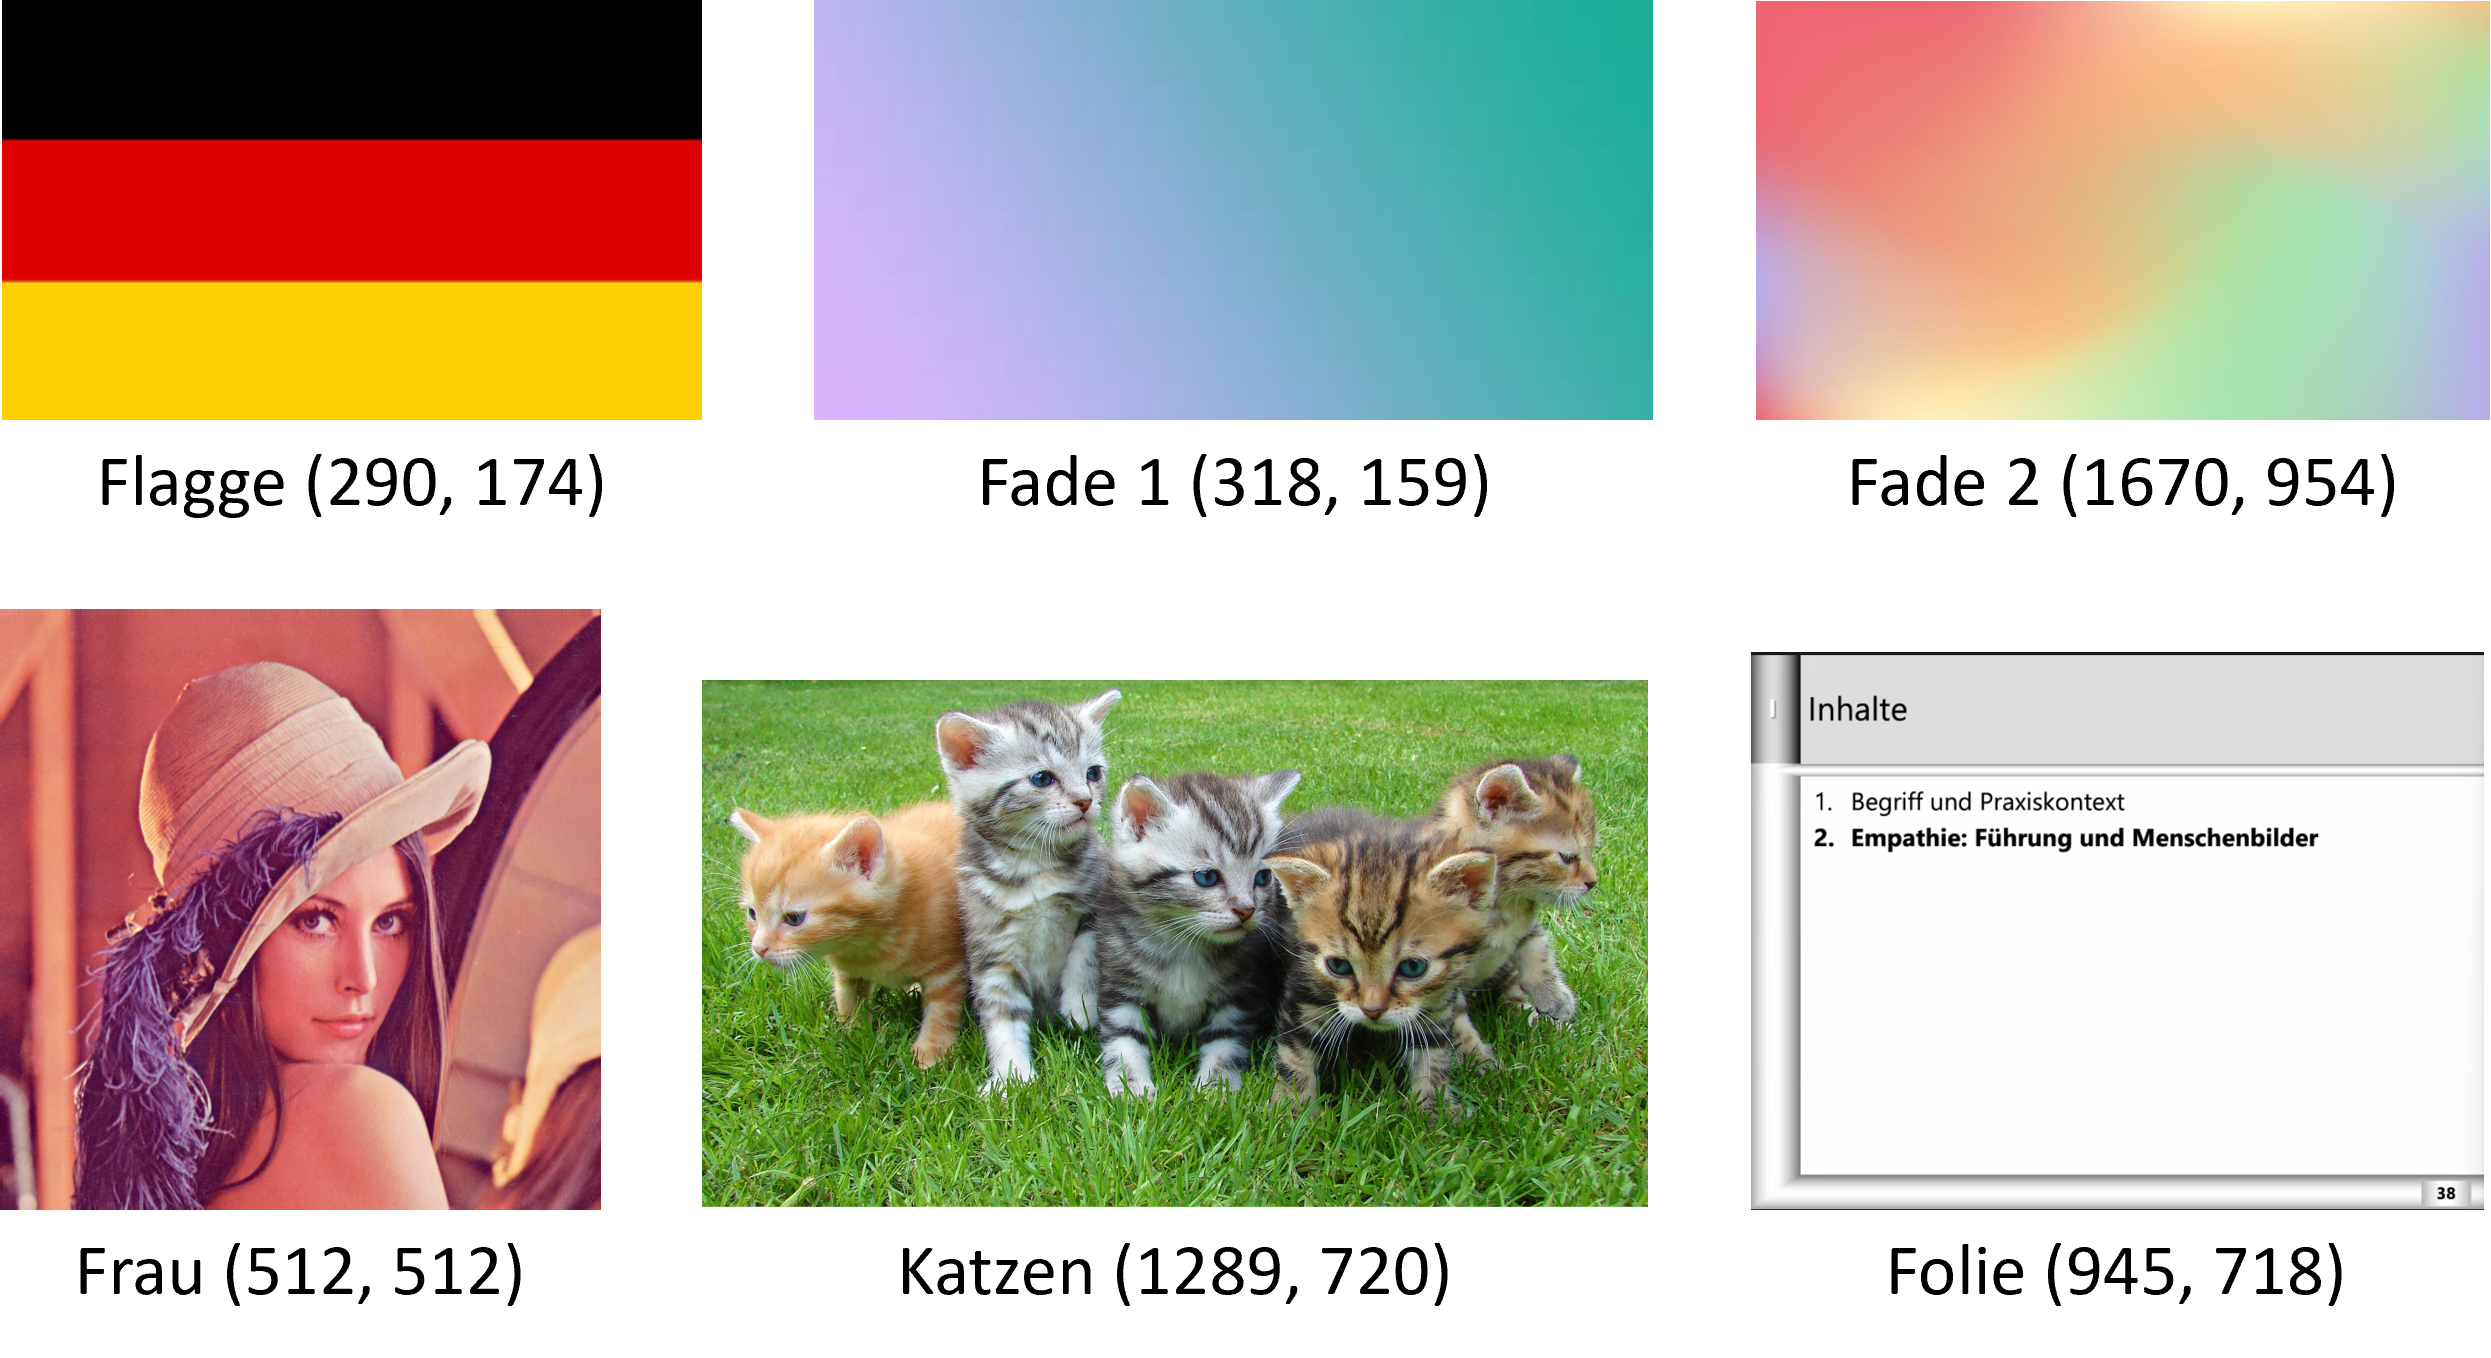
\includegraphics[width=\columnwidth]{./images/Images.png}
  \caption{Testbilder mit Auflösung}
  \label{fig:testbilder}
\end{figure}

Es wurden sehr unterschiedliche Bilder gewählt.
Sie unterscheiden sich sowohl im Motiv als auch in der Bildauflösung.
Die verschiedenen Bildauflösungen wurden gewählt, um die Laufzeit der
Algorithmen auf unterschiedlich großen Eingangsdaten zu vergleichen.
Die Motive sind unterschiedlich aber nicht zufällig gewählt.
Das Bild der Deutschlandflagge und das Bild der Folie haben
viele Bildpunkte mit identischer Farbe.
In den Daten ist viel Redundanz enthalten.
Die Bilder wurden gewählt, da sie aus monotonen Teilbereichen bestehen
und viele Wiederholungen in den Daten vorhanden sind.

Das Bild Fade 1 und Fade 2 zeigen einen Farbverlauf.
Die Daten enthatlten eine große Anzahl an Farbwechsel.
Die Farbwechsel sind nicht zufällig sonder nach einem Farbverlauf Muster.
Fade 1 hat im Großteil des Bildes kaum Rotanteile, während
Fade 2 einen Farbverlauf mit den Grundfarben rot, grün und blau hat.

Das Bild der Frau und das Bild mit den Katzen sind reale Bilder.
Sie zeigen echte Sachverhalte und beschreiben die Struktur
von natürlichen Bilder.


\subsubsection{Erwartungen}

Nach der theoretischen Betrachtung der Algorithmen und der
Datenkompressionsverfahren können einige Erwartungen aufgestellt werden.
Der RLE Algorithmus sollte vor allem bei den Bildern der Flagge und Folie
gut sein, da er Redundanz in Form von Wiederholungen entfernt.
Alle anderen Algorithmen sollten ebenfalls die Redundanz entfernen können.
Die Erwartungen für die Bilder Fade 1 und Fade 2 sind, dass sie standardmäßig
schlecht komprimiert werden könne.
Der Datenvorverarbeitungsschritt mit den Filter sollte zu einer Verbesserung führen.
Bei den natürlichen Bildern sollte vor allem PNG gut funktionieren,
während der RLE Algorithmus schlecht abschneidet.



\section{Ergebnisse und Interpretation}

\subsection{Kompressionsrate}

Die Tabelle \ref{tab:komprate} zeigt die Kompressionsraten der Algorithmen
anhand der Testbilder.
Alle Angaben sind in Prozent und wurden nach der Formel \ref{eq:komprate} berechnet.

\begin{table*}
  \renewcommand*{\arraystretch}{1.1}
  \centering
  \begin{threeparttable}
    \caption{Kompressionsraten}
    \begin{tabular}{c *9{c} S[table-format=5.9]}
      \toprule
      Name         & Auflösung   & RLE    & Huffman & LZ77   & Deflate & Filter + Huffman & Filter + LZ77 & PNG   \\
      \midrule
      Flagge       & (290, 174)  & 99,98  & 77,85   & 78,85  & 91,70   & 87,38            & 84,69         & 91,80 \\
      Fade 1       & (318, 159)  & 45,73  & 14,30   & 25,87  & 31,90   & 84,94            & 78,13         & 80,69 \\
      Frau         & (512, 512)  & -39,19 & 2,74    & -10,96 & -9,51   & 38,22            & -7,41         & 3,38  \\
      Folie        & (945, 718)  & 84,57  & 56,87   & 73,48  & 76,62   & 84,90            & 81,66         & 87,03 \\
      Katzen       & (1289, 720) & -42,85 & 2,11    & -11,39 & -9,31   & 25,49            & -10,42        & -2,45 \\
      Fade 2       & (1670, 954) & 78,95  & 10,95   & 62,13  & 66,95   & 85,74            & 80,59         & 83,74 \\
      \bottomrule
      Durchschnitt &             & 37,87  & 27,47   & 36,33  & 41,40   & 67,78            & 51,21         & 57,37 \\
    \end{tabular}
    \par\tnote{1} Angaben in Prozent, gerundet auf zwei Nachkommastellen
    \par\tnote{2} Bilder nach Größe aufsteigend sortiert
    \label{tab:komprate}
  \end{threeparttable}
\end{table*}

Es können einige generelle Aussagen anhand der Durchschnittswerte gemacht werden.
Alle Kompressionsalgorithmen erreichen im Schnitt eine positive Kompressionsrate von über 20 \%.
Der im Schnitt schlechteste Algorithmus ist Huffman, mit nur 27 \%.
Der im Schnitt beste Kompressionsalgorithmus ist die Kombination aus dem Filtern der Bilddaten
und dem Huffman Algorithmus.
Er erreicht eine Kompressionsrate von 67 \%.


% Auffälligkeiten
% - Huffman schlecht bei Fade, Filter + Huffman krank gut -> Datenvorverarbeitungsschritt
% Filtern, bringt deutliche verbesserung und Erzeugt Redundanz, die vom
% Huffman Algorithmus entfernt werden kann.
% - vlt neg werte

\subsubsection{RLE}

RLE erreicht hohe Kompressionsraten bei computergenerierten Bildern, während natürliche
Bilder kaum oder gar nicht komprimiert werden können.
In der Tabelle ist RLE für die höchste erreichte Kompressionsrate verantwortlich.
Das Bild mit der Flagge kann um 99,98 \% komprimiert werden.
Das Originalbild kann von 151.380 Bytes auf nur 32 Bytes komprimiert werden.
Das Bild besteht aus langen Sequenzen identischer Zeichen. Redundanz in Form von
Wiederholungen wird durch RLE optimal entfernt.

Entgegen den theoretischen Erwartungen ist der Algorithmus auch in der Lage,
Gradientenbilder zu komprimieren. Der Grund dafür liegt in der Struktur der Bilder.
Fade 1 und Fade 2 enthalten Farbkanäle, in denen einige Bereiche viele Wiederholungen aufweisen.
Teilweise bestehen die Farbverläufe nur aus Mischungen von zwei Grundfarben, während der
andere Farbkanal Nullwerte enthält.
Aus diesem Grund kann RLE auch die beiden Bilder mit kontinuierlich wechselnden Farben komprimieren.

Der RLE Algorithmus scheitert an den Testbildern (Frau, Katzen) und erreicht keine
Kompression.
Dies ist daran zu erkennen, dass die Kompressionsraten bei ca. -40 \% liegen, was
bedeutet, dass die kodierten Daten um 40 \% größer sind als die Ausgangsdaten.
RLE scheitert an den Bildern, da es keine offensichtliche Redundanz in Form von Wiederholungen gibt.
Daher nimmt die Kodierung mehr Platz in Anspruch, als sie einspart.


\subsubsection{Huffman}

Der Huffman Algorithmus erreicht im Vergleich zu den anderen Algorithmen keine
hohen Kompressionsraten.
Natürliche Bilder können leicht komprimiert werden, zwischen 2 und 3 \%.
Bilder mit Farbverläufen werden um 10 bis 15 \% komprimiert.
Der Huffman Algorithmus erreicht bei Bildern mit Redundanz in Form von
Wiederholungen Kompressionsraten von über 50 \%.

Eine Schwäche des Algorithmus sind Daten, die viele verschiedene Werte enthalten,
die alle ähnlich häufig vorkommen.
Eine Stärke des Algorithmus ist, dass er stabil ist und positive Kompressionsraten liefert.
Die anderen Algorithmen sind nicht in der Lage, alle Testbilder zu komprimieren.
In der Tabelle ist dies daran zu erkennen, dass keine negativen Werte auftreten.

\subsubsection{Filter + Huffman}

Die Kombination aus Bilddatenfilterung und Huffman Algorithmus erzielt die
beste durchschnittliche Kompressionsrate.
Das Katzenbild wird durch das Verfahren um 25,49 \% komprimiert.
Die erreichte Rate ist mit Abstand die beste aller Algorithmen.
Das Bild der Frau wird durch das Verfahren ebenfalls am besten komprimiert.
Die Kompressionsrate ist um 35 \% besser als die des nächstbesten Algorithmus.
Auch bei den anderen Testbildern erreicht das Verfahren hohe Kompressionsraten von über 84 \%.

Der Datenvorverarbeitungsschritt (Filterung) erzeugt in allen Testbildern Redundanz, die
durch den Huffman Algorithmus effektiv entfernt werden kann.
Der Filter erzeugt Redundanz in Form von Strukturen, wodurch die Anzahl unterschiedlicher
Werte in den Daten reduziert wird.
Das Verfahren ist für alle Arten von Bilddaten geeignet.
Insbesondere natürliche Bilder können mit diesem Verfahren komprimiert werden, während
die anderen Algorithmen versagen.


\subsubsection{LZ77}

Der LZ77 Algorithmus komprimiert die Testbilder Flagge und Folie um 73 \%.
Der Algorithmus ist auch in der Lage, einen Teil der Redundanz in den Gradientenbildern
zu entfernen.
Natürliche Bilder (Frau, Katzen) lassen sich mit LZ77 nicht komprimieren.
Die Kompressionsraten der Bilder liegen bei ca. -11 \%.
Das bedeutet, dass der Algorithmus keine Redundanz entfernen kann und daher die Daten
nicht komprimiert.
Im Gegenteil, der Algorithmus erhöht die Datengröße um 10 \%.
Der LZ77 Algorithmus kann Bilder mit Struktur und Wiederholungen komprimieren.
Er ist jedoch nicht in der Lage, natürliche Bilder zu komprimieren.

\subsubsection{Filter + LZ77}

Die Kombination von Bilddatenfilterung und LZ77 Algorithmus führt zu besseren
Ergebnissen als LZ77 ohne Vorverarbeitungsschritt.
Die Filterung wirkt sich positiv auf die Kompressionsfähigkeit des Algorithmus aus.
Insbesondere beim Testbild Fade 1 entstehen durch die Filterung neue Strukturen,
die durch den LZ77 Algorithmus entfernt werden können.
Die Kompressionsrate verbessert sich durch den Vorverarbeitungsschritt um 52 \%.
Durch die Filterung entstehen Strukturen, da die Filter die Daten in
Relativwerte zu den Nachbarwerten umwandeln.
In ungefilterten Bildern sind die Strukturen Absolutwerte der Pixel.
Die Filterung erzeugt durch Relativwerte wiederkehrende Muster aus einem Farbverlauf.
Bei natürlichen Bildern versagt der Algorithmus und es wird eine
Kompressionsrate von -9 \% erreicht.


\subsubsection{Deflate (LZ77 + Huffman)}

Der Deflate Algorithmus schneidet bei den gleichen Testbildern gut ab, bei
denen RLE gut ist.
Das bedeutet, dass der Deflate Algorithmus Wiederholungen effektiv entfernt.
Der Deflate Algorithmus ist für jedes Bild besser als der LZ77 Algorithmus.
Daraus folgt, dass LZ77 nicht die gleiche Redundanz erkennt wie Huffman.
Die Daten enthalten nach der Kodierung mit dem LZ77 Algorithmus weitere
Redundanz, die mit dem Huffman Algorithmus entfernt werden kann.

Der Deflate Algorithmus hat die gleichen Stärken und Schwächen wie der LZ77 Algorithmus.
Für natürliche Bilder (Frau, Katzen) erreicht das Verfahren eine negative
Kompressionsrate von -9 \%.

\subsubsection{PNG (Filter + Deflate)}

Die Vorverarbeitung der Daten mit den Filtern führt bei allen Bilddaten zu einer
Verbesserung gegenüber dem Deflate-Algorithmus.
Insbesondere das Testbild Fade 1 erreicht durch die zusätzliche Filterung
eine deutlich höhere Kompressionsrate.
Der Grund dafür ist, dass durch das Filtern absolute Pixelwerte in relative Werte
umgewandelt werden.
Dadurch werden Strukturen im Gradientenbild sichtbar.

Das Bild der Frau erreicht eine Kompressionsrate von etwas über 3 \%.
Dies ist eine deutliche Verbesserung gegenüber den -9 \% des Deflate Algorithmus.
Für strukturierte Daten und Daten mit Wiederholungen funktioniert der
PNG Algorithmus gut und erreicht Kompressionsraten von über 80 \%.
Lediglich das Katzenbild kann nicht komprimiert werden.


\subsubsection{Fazit Kompressionsraten}

Aus dem Vergleich der Kompressionsraten wurden einige Erkenntnisse gewonnen werden.
Der Datenvorverarbeitungsschritt mit den Filter liefert für alle getesteten
Algorithmen eine Verbesserung in der Kompressionsrate.
Das beweist, dass das Filtern Redundanz erzeugt, die im nächsten Schritt
entfernt werden kann.
Das Filtern von Bilddaten ist als Vorverarbeitungsschritt effektiv.


Der PNG Algorithmus ist in der Praxis schlechter als theoretisch angenommen.
Das Verfahren schafft es nicht alle Testbilder erfolgreich zu komprimieren.
Ein Grund für die Ergebnisse können mit der Implementierung des
LZ77 Algorithmus Zusammenhängen.
Bei der Implementierung wurde die Größe des Sliding Window auf 100 festgelegt.
Das ist deutlich kleiner als die in der Spezifikation maximal angegebene Größe.
Sie ist 32768. \cite{w3c}

Bei strukturierten Daten mit vielen Wiederholungen ist RLE eine valide
Option und erreicht Teilweise sogar die besten Kompressionsraten.
Das allgemein beste getestete Kompressionsverfahren für Bilder ist die Kombination
aus Filtern der Daten gefolgt von dem Huffman Algorithmus.

Zusammenfassend kann festgehalten werden, dass die Kompressionsraten
stark von den Bilder selbst abhängen.
Sturkturierte Bilder können stark komprimiert werden wo hingegen natürlichen Bilder
zu einem kleineren Teil komprimiertbar sind.
Kein Kompressionsverfahren ist für alle Bilder am besten und es macht Sinn
mehrere zu vergleichen, welches für ein konkretes Bild am effektivsten ist.


\subsection{Kompressionszeit und Dekompressionszeit}

Die Ergebnisse der Kompressions- und Dekompressionszeiten sind stark
hardware- und implementierungsabhängig.
Daher wird nicht explizit auf die absoluten Zeiten eingegangen.
Es geht darum, Tendenzen aufzuzeigen und die Algorithmen miteinander zu vergleichen.

\begin{table*}
  \renewcommand*{\arraystretch}{1.1}
  \centering
  \begin{threeparttable}
    \caption{Kompressionszeiten}
    \begin{tabular}{c *9{c} S[table-format=5.9]}
      \toprule
      Name   & Auflösung   & RLE   & Huffman & LZ77 & Deflate & Filter + Huffman & Filter + LZ77 & PNG & Filter \\
      \midrule
      Flagge & (290, 174)  & 0,015 & 0,017   & 2,3  & 2,3     & 1,3              & 3,3           & 3,3 & 1,3    \\
      Fade 1 & (318, 159)  & 0,028 & 0,018   & 14   & 14      & 1,6              & 5             & 5   & 1,6    \\
      Frau   & (512, 512)  & 0,21  & 0,09    & 139  & 139     & 9                & 131           & 131 & 9      \\
      Folie  & (945, 718)  & 0,47  & 0,24    & 63   & 63      & 22               & 62            & 62  & 22     \\
      Katzen & (1289, 720) & 0,77  & 0,33    & 530  & 530     & 32               & 540           & 540 & 32     \\
      Fade 2 & (1670, 954) & 0,61  & 0,55    & 200  & 200     & 51               & 140           & 140 & 51
    \end{tabular}
    \par\tnote{1} Angaben in Sekunden
    \par\tnote{2} Bilder nach Größe aufsteigend sortiert
    \par\tnote{3} Die Spalte Filter gibt die Filterzeit an
    \label{tab:kompzeiten}
  \end{threeparttable}
\end{table*}

Die Kompressionszeiten der Algorithmen sind in der
Tabelle \ref{tab:kompzeiten} aufgelistet.
Die Tabelle ist aufsteigend nach Auflösung bzw. Datengröße sortiert.
Aus den Ergebnissen können einige Schlussfolgerungen gezogen werden.

RLE hat eine lineare Laufzeitkomplexität, was durch die Ergebnisse
praktisch bestätigt wird.
Jedes Bild kann in weniger als 1 Sekunde komprimiert werden.
Der Huffman Algorithmus hat ebenfalls eine lineare Laufzeitkomplexität
und ist in der Praxis etwas schneller.


LZ77 hat eine Laufzeitkomplexität von $O(n * s)$.
Die Messungen zeigen, dass die Implementierung von LZ77 deutlich
langsamer komprimiert als RLE oder Huffman.
Ebenso können Ausreißer wie im Bild mit den Katzen beobachtet werden.

Die Laufzeit hängt direkt damit zusammen, wie weit LZ77 durch das
Sliding Window iterieren muss, um einen Treffer zu finden.
Das Katzenbild enthält deutlich unstrukturiertere Daten als das Bild
Fade 2.
Beim Katzenbild wird deutlich länger im Sliding Window gesucht um
einen Treffer zu finden oder es wird kein Treffer gefunden.

Das Filtern eines Bildes benötigt lineare Zeit und ist unabhängig
von der Struktur des Bildes.
D.h. egal wie das Bild aufgebaut ist, die Laufzeit für das Filtern
hängt nur von der Größe des Bildes ab.

Das Verfahren Filter + LZ77 ist etwas schneller als LZ77 ohne Vorverarbeitung.
Dies liegt daran, dass die Daten nun stärker komprimiert werden können und
weniger weit durch das Sliding Window iteriert werden muss, um eine
Übereinstimmung zu finden.

Die Laufzeit von Filter + Huffman ist fast identisch mit der Laufzeit
für das Filtern.
Der Grund dafür ist, dass der Huffman-Algorithmus die Daten sehr
schnell komprimiert.
Die Kompressionszeit des Deflate- und PNG Algorithmus entspricht
weitgehend der Laufzeit des LZ77 Algorithmus.
LZ77 ist für die langen Kompressionszeiten verantwortlich.


\begin{table*}
  \renewcommand*{\arraystretch}{1.1}
  \centering
  \begin{threeparttable}
    \caption{Dekompressionszeiten}
    \begin{tabular}{c *9{c} S[table-format=5.9]}
      \toprule
      Name   & Auflösung   & RLE   & Huffman & LZ77  & Deflate & Filter + Huffman & Filter + LZ77 & PNG   & Revert Filter \\
      \midrule
      Flagge & (290, 174)  & 0,003 & 0,012   & 0,120 & 0,124   & 0,124            & 0,255         & 0,255 & 0,120         \\
      Fade 1 & (318, 159)  & 0,032 & 0,048   & 3,5   & 3,5     & 0,008            & 0,500         & 0,550 & 0,220         \\
      Frau   & (512, 512)  & 0,395 & 0,293   & 308   & 308     & 1,4              & 230           & 230   & 1,4           \\
      Folie  & (945, 718)  & 0,769 & 0,321   & 82    & 82      & 3                & 35            & 35    & 2,9           \\
      Katzen & (1289, 720) & 1,4   & 1       & 1200  & 1200    & 5,1              & 1205          & 1205  & 5             \\
      Fade 2 & (1670, 954) & 0,480 & 1,5     & 732   & 732     & 7                & 184           & 184   & 7
    \end{tabular}
    \par\tnote{1} Angaben in Sekunden
    \par\tnote{2} Bilder nach Größe aufsteigend sortiert
    \par\tnote{3} Die Spalte Revert Filter gibt die Zeit an, in der die Filterung rückgängig gemacht wird
    \label{tab:dekompzeiten}
  \end{threeparttable}

\end{table*}

Die Dekompressionszeiten der Algorithmen sind in der Tabelle
\ref{tab:kompzeiten} aufgelistet.
Das Rückgängigmachen der Filteroperation (Revert Filter) ist
schneller als das Filtern.
Revert Filter hat eine Laufzeitkomplexität von $O(n)$, während das Filtern
$O(5n)$ benötigt.
In der Theorie ist $O(n) = O(5n)$, aber in der Praxis spielt der
Vorfaktor eine Rolle.
In der Praxis ist das Filtern sogar um den Faktor 9 schneller.
Dies ermöglicht eine schnellere Dekompression als Kompression.

Die Laufzeit der RLE-Dekompression hängt stark von den Daten ab.
Wenn die Daten stark komprimiert sind, ist der Dekompressionsschritt
schnell, da die Rekonstruktion von Wiederholungen schnell ist.
Die Dekompression des Huffman Algorithmus ist etwas langsamer
als die Kompression.
Die Dekompressionszeit des LZ77 Algorithmus variiert und hängt
stark von den Daten ab.
Je besser die Bilder komprimiert werden können, desto schneller
ist die Dekompression im Verhältnis zur Bildgröße.
Die Dekompressionszeit des Deflate- und des PNG Algorithmus entspricht
weitgehend der des LZ77 Algorithmus.
LZ77 ist für die langen Dekompressionszeiten verantwortlich.

Aus den Tabellen können einige Schlüsse gezogen werden.
Der Huffman- und der RLE Algorithmus sind schnell in Bezug auf die
Kompressions- und Dekompressionszeit.
Das Filtern eines Bildes erfolgt in linearer Laufzeit.
Das Rückgängigmachen des Filterns während der Dekompression ist um
den Faktor 9 schneller als das Filtern selbst.
RLE, Huffman und Filter sind auch ohne Optimierung der Implementierung
geeignet, Bilder in akzeptabler Zeit zu komprimieren und zu dekomprimieren.
Jedes Verfahren, das den LZ77 Algorithmus verwendet, ist ohne Optimierung
nicht geeignet, da die Laufzeit deutlich länger ist als bei anderen Verfahren.
Ebenso ist LZ77 für hochaufgelöste Bilddaten langsam.

Aus der Abwägung zwischen Kompressionsrate und Laufzeit ergibt sich, dass
Filter + Huffman das beste Verfahren ist.
Abhängig von der Struktur der zu komprimierenden Bilder kann der RLE
Algorithmus eine Alternative sein.
LZ77, Deflate und PNG sind aufgrund der vergleichsweise schlechten Performance
des LZ77 Algorithmus in Bezug auf Kompressionsrate und Laufzeit nicht geeignet.
Um mit diesen Verfahren bessere Ergebnisse zu erzielen, muss das Sliding Window
deutlich vergrößert und eine effizientere Implementierung verwendet werden.


\section{Fazit}

Die Ergebnisse des praktischen Versuchs entsprachen nicht den Erwartungen.
Nicht der PNG Algorithmus, sondern das Filtern mit anschließendem
Huffman Algorithmus erzielt die besten Kompressionsraten.
Insbesondere die Vorverarbeitung der Bilder mit den Filtern führt
bei allen Kompressionsalgorithmen zu einer deutlichen Verbesserung
der Kompressionsrate.
Auch bei den Laufzeiten für Kompression und Dekompression schneiden
Huffman, RLE und der Vorverarbeitungsschritt gut ab.
Die Verfahren ermöglichen auch ohne optimierte Implementierung der
Algorithmen eine effektive Bildkompression und -dekompression bei
geringer Laufzeit.
Der PNG-, der Deflate- und der LZ77 Algorithmus sind in ihrer Laufzeit und
Kompressionsfähigkeit eingeschränkt.
Die Gründe hierfür liegen in der Implementierung des LZ77 Algorithmus und
wurden in den vorherigen Kapiteln beschrieben.

Bei komplexen Bildern ohne erkennbare Struktur versagen einige Algorithmen.
Nur der Filter + Huffman Algorithmus kann alle getesteten Bilder erheblich
komprimieren.
Die Komprimierbarkeit von Bildern hängt stark vom Bild selbst ab.
Außerdem gibt es nicht ein Verfahren, das jedes Bild am besten komprimiert.
Jedes Verfahren entfernt verschiedene Redundanzen unterschiedlich gut.

\bibliographystyle{IEEEtran}
\bibliography{mybib}

\end{document}
